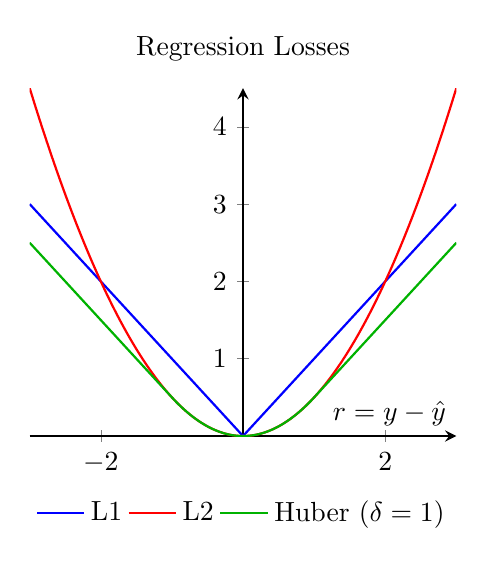
\begin{tikzpicture}
    % ---------------- Left plot: L1, L2, Huber ----------------
    \begin{axis}[
            name=regression,
            at={(0,0)}, anchor=north west,
            xlabel={$r = y - \hat{y}$},
            % ylabel={Loss},
            % grid=major,
            axis lines=middle,
            domain=-3:3,
            samples=200,
            legend style={at={(0.5,-0.15)}, anchor=north, draw=none, legend columns=3},
            width=7cm, height=6cm,
            thick,
            title={Regression Losses}
        ]
        \addplot[blue] {abs(x)};
        \addlegendentry{L1}
        \addplot[red] {0.5*x^2};
        \addlegendentry{L2}
        \addplot[green!70!black] {abs(x) < 1 ? 0.5*x^2 : 1*(abs(x)-0.5*1)};
        \addlegendentry{Huber ($\delta=1$)}
    \end{axis}
\end{tikzpicture}
% ---------------- Right plot: Cross-Entropy ----------------
\hspace{1cm}
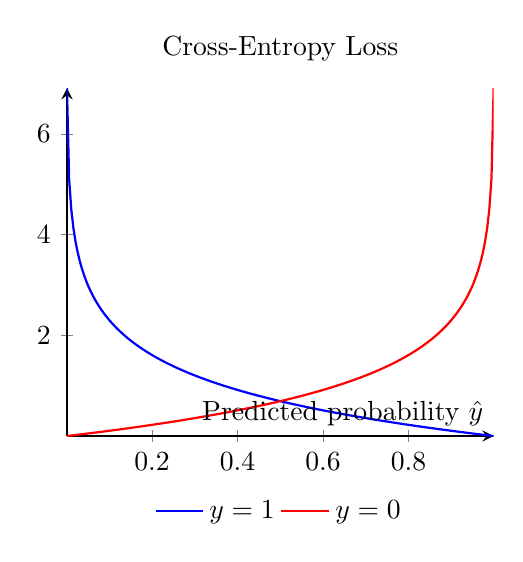
\begin{tikzpicture}
    \begin{axis}[
            xlabel={Predicted probability $\hat{y}$},
            % ylabel={Cross-Entropy Loss},
            % grid=major,
            axis lines=middle,
            domain=0.001:0.999,
            samples=200,
            width=7cm,
            height=6cm,
            thick,
            legend style={at={(0.5,-0.15)}, anchor=north, draw=none, legend columns=2},
            title={Cross-Entropy Loss}
        ]

        % y = 1
        \addplot[blue] {-ln(x)};
        \addlegendentry{$y=1$}

        % y = 0
        \addplot[red] {-ln(1-x)};
        \addlegendentry{$y=0$}
    \end{axis}
\end{tikzpicture}